% !Mode:: "TeX:UTF-8"
% Author: Zhengxi Tian
% Email: zhengxi.tian@hotmail.com

\chapter{相关工作}\label{ch:related_work}
\section{生成式模型}\label{sec:generative_model}
一个生成式模型定义了给定输入序列$X = x_1, x_2, \cdots, x_n$,
任意输出序列$Y = y_1, y_2, \cdots, y_m$的条件概率:
\begin{align}
    p(Y|X) = P(y_1, y_2, \cdots, y_m|x_1, x_2, \cdots, x_n)
    \label{eqn:generative_conditional_probability}
\end{align}
模型的训练目标就是在数据集$S$上最大化给定$X$,$Y$的对数概率(Log Probability):
\begin{align}
    \mathit{L} = \frac{1}{|S|} \sum_{(Y, X) \in S} \log p(Y|X)
\end{align}
从这个角度来看,语言模型\upcite{
DBLP:journals/jmlr/BengioDVJ03,
DBLP:conf/interspeech/MikolovKBCK10}(Language Model)和编解码器(Encoder-Decoder)都属于生成式模型,
因为它们都定义了条件概率$p(Y|X)$。
生成式模型把一个长度可变的序列$X$映射到另一个长度可变的序列$Y$,且$X$和$Y$的长度可以不相等。
循环神经网络(RNN)为这个问题提供了自然的解决方案。
% RNN
RNN的基本思想是:序列由有序的元素组成,每一个时刻(Time Step)输入并输出一个元素,同时更新内部的隐层状态(Hidden State)。
在时间轴上展开的RNN和一般的前馈神经网络(Feed Forward Neural Networks)很像,不过每一个时刻的权重矩阵都是共享的。
这个共享的权重矩阵$A$又被称为循环矩阵(Recurrent Matrix)。
循环矩阵的作用是保存输入序列的顺序信息,并把当前时刻的输入序列编码成一个定长向量。
图~\ref{fig:RNN_unrolled}\footnote{http://colah.github.io/posts/2015-08-Understanding-LSTMs/}
描绘了简化的RNN结构。
\begin{figure}[H]
    \centering
    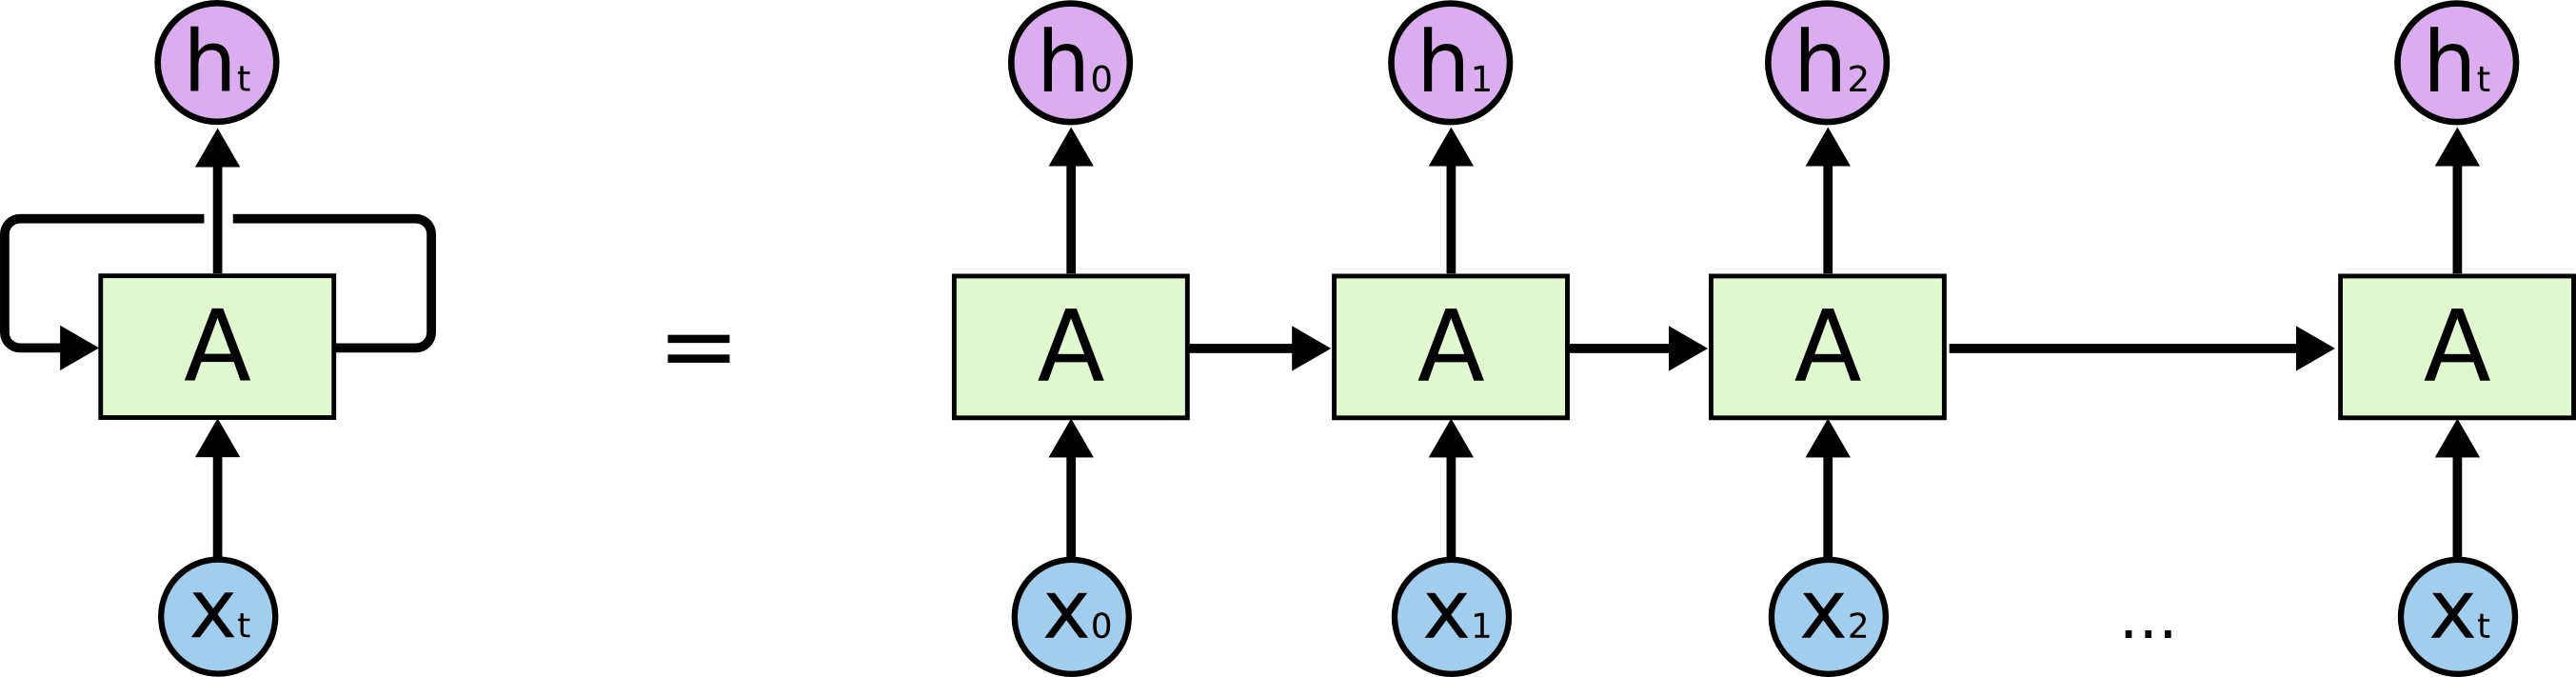
\includegraphics[width=0.6\textwidth]{figure/RNN-unrolled.png}
    \caption{RNN的一般表示和展开表示}
    \label{fig:RNN_unrolled}
\end{figure}

% RNN细分
根据是否使用了某种门单元,RNN可分为普通RNN\upcite{DBLP:conf/interspeech/MikolovKBCK10},
LSTM\upcite{DBLP:journals/neco/HochreiterS97}和GRU\upcite{DBLP:conf/emnlp/ChoMGBBSB14}。
根据是否对反向序列(Reversed Sequence)建模,RNN可分为单向RNN(Unidirectional RNN)
和双向RNN(Bidirectional RNN)\upcite{DBLP:journals/tsp/SchusterP97}。
由于普通RNN受到梯度消失的影响,目前学界普遍采用LSTM或者GRU;
尽管后者受到梯度爆炸的影响,但是可以通过梯度剪裁(Gradient~Clipping)
\upcite{DBLP:journals/corr/VinyalsL15}解决。
采用多层RNN组成的深度神经网络比单层RNN能获得更好的性能\upcite{DBLP:journals/corr/VinyalsL15}。

% RNNLM
RNN语言模型可以给出序列$X=x_1, x_2, \cdots, x_n$的概率分布:
\begin{align}
    p(X) = \prod_{i=1}^{n} p(x_i|x_1, x_2, \cdots, x_{i-1})
    \label{eqn:language_model_probability}
\end{align}

RNN语言模型\footnote{为了简洁起见,我们描述了普通RNN。LSTM和GRU有着更复杂的数学表达式。}
通过神经网络中的参数来估计公式~\ref{eqn:language_model_probability}~乘积中的一项:
\begin{align}
    p(x_i = w|x_1, x_2, \cdots, x_{i-1}) = \frac{\exp{o_{tw}}}{\sum_{v=1}^V \exp{o_{tv}}}
    \label{eqn:language_model_estimation}
\end{align}
$o_t$是RNN的在$t$时刻的输出向量,$V$是词汇表的大小。
公式~\ref{eqn:language_model_estimation}~的右边本质上是对一个长度为$V$的向量进行softmax运算。
$t$时刻的输出向量是由输出矩阵$W_{out}$和$t$时刻隐层状态$h_i$相乘得到的:
\begin{align}
    o_i &= h_i^T W_{out}
\end{align}
而$h_i$则是当前输入$x_i$和上一时刻的隐层状态$h_{i-1}$在输入矩阵$W_{in}$和循环矩阵$W_{hh}$分别作用后再相加的结果:
\begin{align}
    h_i &= \sigma \left( x_i^T W_{in} + h_{i-1}^T W_{hh} \right)
\end{align}
RNN语言模型在训练时最大化训练集上的句子的对数概率:
\begin{align}
    \mathit{L(X)} = \sum_{i=1}^n \log p(x_i|x_1, x_2, \cdots, x_{i-1})
\end{align}
在预测时,对模型输入消息$m$,从模型的给出的概率分布中用某种搜索方法,如Beam Search可得出响应$r$。

% Seq2Seq
Seq2Seq框架使用两个拥有独立参数的RNN分别作为编码器和解码器。
尽管编解码器不一定都使用RNN\upcite{DBLP:journals/corr/BahdanauCB14},本文仅关注使用RNN的Seq2Seq变体。
首先,编码器把输入序列$X$编码成一个定长向量$v$。
该向量又称为思考向量(Though Vector),是编码器完全读取输入序列后的隐层状态(Last Hidden State)。
接着,解码器以$v$为初始隐层状态(Initial Hidden State),像一个RNN语言模型一样对输出序列进行预测。
整个过程可以描述为:编码器把输入序列$X$变换成某种压缩编码$v$,再由解码器把$v$还原为另一个序列$Y$,
Seq2Seq把公式~\ref{eqn:generative_conditional_probability}~
作了如下转化:
\begin{align}
    p(y_1, y_2, \cdots, y_m|x_1, x_2, \cdots, x_n) = \prod_{i=1}^m p(y_i|v, y_1, y_2, \cdots, y_{i-1})
\end{align}
其中$v$是以$f$为门单元的编码器的最后一个隐层状态:
\begin{align}
    h_i &= f(x_i ,h_{i-1}) \\
    c &= h_n
\end{align}
编码器和解码器以同一个目标函数同时训练。
为了更好的处理长序列,Seq2Seq一般引入注意力机制(Attention Mechanism)
\upcite{
    DBLP:journals/corr/BahdanauCB14,
    DBLP:conf/emnlp/LuongPM15},使输入序列的信息不必全部通过固定长度的向量$v$传递。
解码器能自动关注和当前输出最相关的输入部分,实现输入序列与输出序列的对齐(Alignment)。
注意力机制使传统Seq2Seq模型对较长输入也具有鲁棒性。

% Beam Search,Greedy & Random Sample
生成式模型仅仅定义了条件概率$p(Y|X)$,在推理阶段(Inference),需要采用某种启发式搜索算法从概率分布中
生成输出$Y$,这个过程又称为解码(Decode)。
最简单的搜索算法是贪心搜索(Greedy Search):在每一时刻都输出条件概率最大的单词:
\begin{align}
    y_i = \argmax p(y_i|y_1, y_2, \cdots, y_{i-1}|X)
\end{align}
因为各个$y_i$的概率都不是独立的,而是受之前输出的单词的影响,贪心搜索不能保证得到概率最大的输出序列。
随机取样(Random Sampling)在每一时刻都从模型生成的全体词汇的概率分布中随机选取一个单词。
这样输出就带有一点不确定性,在一定程度上增加了输出的多样性。
最为常用的是集束搜索(Beam Search),它在生成整个句子的过程中维护一个大小为$B$的列表,称为集束(Beam)。
算法开始时,集束初始化为模型生成的$B$个概率最高的单词。
在每一个时刻开始时,集束中都有$B$个部分生成的句子,它们称为候选$Y_c$。
在每一个时刻,算法对集束中的每一个候选都生成$B$个概率最大的下一个单词$w_{i+1, c}$,从而形成$B \times B$个部分生成的句子$Y_{ex}$,
称为扩展的候选集。从扩展的候选集中,只保留前$B$个概率$p(Y_{ex}|X)$最大的句子。
算法不断迭代直到在某次对候选集的扩展中,某些候选中产生了句子结束符号(End-of-Sentence,EOS),
于是概率最大而且完成了的候选句子将作为输出。

% Diverse Beam
为了增加模型输出的多样性,不少学者提出了改进的解码算法。
Li等人提出在标准集束搜索中,对来自相同父节点的候选加以惩罚,换句话说,鼓励来自不同父节点的候选\upcite{DBLP:journals/corr/LiMJ16}。
%Li等人还提出了用最大互信息(MMI)对

% Hierarchical

\section{自动化评价指标}\label{sec:automatic_metric}

\section{公开的对话数据集}\label{sec:public_dataset}

\section{本章小结}\label{sec:rw_conclusion}
%这一节总结所有提及的指标,给它们分一下类,然后简要说明每一类
%指标的特点,或者是它考察的方面。
